\documentclass[notheorems,mathserif,table,compress]{beamer}  %dvipdfm选项是关键,否则编译统统通不过
%%------------------------常用宏包------------------------
%%注意, beamer 会默认使用下列宏包: amsthm, graphicx, hyperref, color, xcolor, 等等
\usepackage{fontspec,xunicode,xltxtra}  % for XeTeX
\usepackage{subfigure} %%图形或表格并排排列
%\usepackage{colortbl,dcolumn}     %% 彩色表格
\usepackage{styles/zhfontcfg}
%\usepackage{styles/iplouclistings}
%\usepackage{listings}
%\usepackage{styles/iplouccfg}
\usepackage{comment}
\usepackage{fancybox}



%%------------------------ThemeColorFont------------------------
%% Presentation Themes
% \usetheme[<options>]{<name list>}
\usetheme{Madrid}
%% Inner Themes
% \useinnertheme[<options>]{<name>}
%% Outer Themes
% \useoutertheme[<options>]{<name>}
\useoutertheme{miniframes} 
%% Color Themes 
% \usecolortheme[<options>]{<name list>}
%% Font Themes
% \usefonttheme[<options>]{<name>}
\setbeamertemplate{background canvas}[vertical shading][bottom=white,top=structure.fg!7] %%背景色, 上25%的蓝, 过渡到下白.
\setbeamertemplate{theorems}[numbered]
\setbeamertemplate{navigation symbols}{}   %% 去掉页面下方默认的导航条.

%\setsansfont[Mapping=tex-text]{文泉驿正黑}  %% 需要fontspec宏包
     %如果装了Adobe Acrobat,可在font.conf中配置Adobe字体的路径以使用其中文字体
     %也可直接使用系统中的中文字体如SimSun,SimHei,微软雅黑 等
     %原来beamer用的字体是sans family;注意Mapping的大小写,不能写错
     %设置字体时也可以直接用字体名,以下三种方式等同:
     %\setromanfont[BoldFont={黑体}]{宋体}
     %\setromanfont[BoldFont={SimHei}]{SimSun}
     %\setromanfont[BoldFont={"[simhei.ttf]"}]{"[simsun.ttc]"}
%%------------------------MISC------------------------
\graphicspath{{figures/}}         %% 图片路径. 本文的图片都放在这个文件夹里了.
%%------------------------正文------------------------
\begin{document}
\XeTeXlinebreaklocale "zh"         % 表示用中文的断行
\XeTeXlinebreakskip = 0pt plus 1pt % 多一点调整的空间
%%----------------------------------------------------------
%% This is only inserted into the PDF information catalog. Can be left
%% out.
%%%
%% Delete this, if you do not want the table of contents to pop up at
%% the beginning of each subsection:
\begin{comment}
\AtBeginSection[]{                              % 在每个Section前都会加入的Frame
  \frame<handout:0>{
    \frametitle{Content}\small
    \tableofcontents[current,currentsubsection]
  }
}
\AtBeginSubsection[]                            % 在每个子段落之前
{
  \frame<handout:0>                             % handout:0 表示只在手稿中出现
  {
    \frametitle{下一节内容}\small
    \tableofcontents[current,currentsubsection] % 显示在目录中加亮的当前章节
  }
}
\end{comment}
%%----------------------------------------------------------
\title{科研总结与展望}
\author[zhu]{主讲人~~~~~\textcolor{olive}{朱亚菲}\\
    \quad 幻灯片制作~~\textcolor{olive}{朱亚菲}}
\institute[中国海洋大学]{\small\textcolor{violet}{中国海洋大学~~信息科学与工程学院}}
\date{2015~年~2~月~2~日}
\frame{ \titlepage }
%%----------------------------------------------------------
%\section*{目录}
\frame{\frametitle{目录}\tableofcontents}
%%----------------------------------------------------------

%\section{Beamer类和XeTeX概览} %如果你想书签不出现问题,请不要用\XeTeX
                                 %这类复杂的指令,直接写XeTeX吧






\section{最新科研内容}

\subsection{November}


\begin{frame}
  \frametitle{SPIC论文投稿}
  \centering\includegraphics[width=3.5in]{zhm.eps}
\end{frame}


\begin{frame}
\frametitle{存在的问题}
\begin{itemize}
\item 目前没有什么方法能较准确地找到显著目标的大小
\item 在HFT方法的基础上改进,效果改善不明显,在HFT与我们的方法中都采用同样的后续处理步骤(Smooth,BorderCut,CenterBias),在有的数据集上pr评价效果甚至不如HFT
\end{itemize}
\end{frame}


\begin{frame}
\frametitle{实验与结论}
实验
\begin{itemize}
\item 取少量背景简单的测试图像(取了100幅),用不同的滤波参数(sigma值不同)对其进行滤波,看滤波参数与其中显著目标(通过Groundtruth可以求得)的关系(例如将滤波参数用长、宽的最大值或最小值、长和宽的乘积等求出的一个公式来表示)
\end{itemize}
结论
\begin{itemize}
\item 显著目标特别大(包含像素超过整幅图像像素个数的40\%)时,一般需要用一个较大 的参数(sigma取100-1000,效果基本一样);而当显著目标不是很大时,情况变得较为复杂,有时需要小参数,有时需要大参数,很难只根据显著目标大小来判断,初步判断还会与前景背景的可分离度有关。
\end{itemize}
\end{frame}


\subsection{December}

\begin{frame}
\frametitle{再次实验}
\begin{itemize}
\item 尝试用其它的滤波器(例如log-Gabor),自己构造滤波器,并且不对幅度谱进行滤波了,而是直接对原图像滤波
\item 不用四元傅里叶变换,而对图像的每个通道分别进行傅里叶变换
\item 改变四元傅里叶部分的特征输入
\item 先进行超像素分割,再做后续处理
\item \ldots
\end{itemize}
\end{frame}

\subsection{January}

\begin{frame}
\frametitle{超像素分割}
\begin{description}
\item[产生背景] 
\begin{itemize}
\item 人类视觉感知单元
\item 数码产品的不断更新
\end{itemize}
\end{description}

\begin{description}
\item[超像素] 超像素\footnote{Xiaofeng Ren and Jitendra Malik. Learning a classification model for segmentation. In Computer Vision, 2003. Proceedings. Ninth IEEE International Conference on, pages 10–17. IEEE, 2003.}是指具有相似纹理、颜色、亮度等特征的相邻像素构成的图像块。这些图像块大都没有破坏图像的边界信息,而且还保留了对图像进行进一步分割的有效信息。
\end{description}
\end{frame}


\begin{frame}
\frametitle{超像素分割}
\begin{figure}
  \centering 
  \subfigure[]{ 
    \label{fig: TurboPixels: a} %% label for first subfigure 
    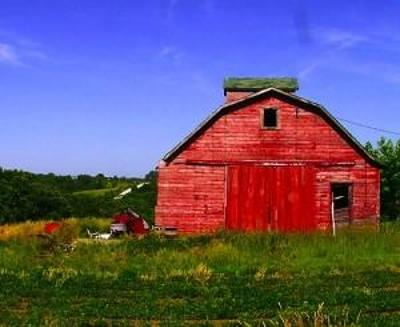
\includegraphics[width=0.4\textwidth]{example1.jpg}} 
  \subfigure[]{ 
    \label{fig: TurboPixels: b} %% label for second subfigure 
    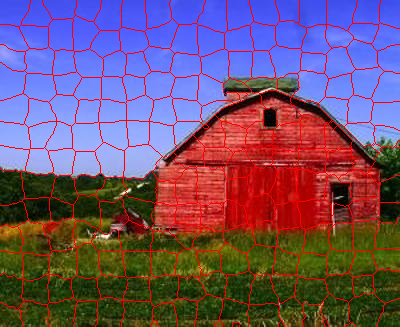
\includegraphics[width=0.4\textwidth]{TurboPixels1.png}}  
  \caption{TurboPixels: $N_{sp}$ = 200}
  \label{fig: TurboPixels} %% label for entire figure
\end{figure}
\end{frame}


\begin{frame}
\frametitle{超像素分割}
超像素分割算法大致可分为基于图论的方法和基于梯度上升的方法两类。
\end{frame}


\begin{frame}
  \frametitle{基于图论的方法}
  基于图论的超像素分割方法将图像看做一幅带权无向图,图像中每一个像素对应图中的每一个节 点,像素之间的相邻关系(通常是 4-邻接或者 8-邻接)对应图的边,像素特征之间的差异或相似性对 应边上的权重。将图像映射为图后,图像分割过程可以看作是根据像素的特征信息,对每一个像素分 配标记的过程,相同特性的像素具有相同的标记,不同特性的像素具有不同的标记。
\end{frame}


\begin{frame}
  \frametitle{基于梯度上升的方法}
  梯度上升方法是从一个粗糙的像素的初始聚类开始,通过不断的迭代来优化聚类簇,直至满足收 敛准则以形成超像素。
\end{frame}


\begin{frame}
  \frametitle{特征总结}
  图像特征提取是图像分析与图像识别的前提,它是将高维的图像数据进行简化表达最有效的方式, 从一幅图像的 $M \times N \times 3$ 的数据矩阵中,我们看不出任何信息,所以我们必须根据这些数据提取出 图像中的关键信息,一些基本元件以及它们的关系。
\end{frame}

\begin{frame}
  \frametitle{特征总结}
图像特征可分为全局特征和局部特征。其最大的区别是特征提取的空间范围不同。全局特征是从 整个图像中提取的特征,而局部特征是从图像区域中提取的特征。

在显著性检测中,由于关注的是显著目标,并且是在同一幅图像中进行中央 -周围/局部/全局对比, 而不是在图像间进行比较,因此用到的应该都是局部特征。显著性检测领域所说的局部和全局方法是 指对某一像素或区域,在计算其对比度时是与周围相比还是与图像中所有其它像素或区域相比。
\end{frame}


\section{所有工作内容}

\begin{frame}
  \frametitle{}
  研一
  \begin{itemize}
  \item 学习数值分析、数字图像处理、网络公开课,初步掌握了git、matlab、c的使用
  \end{itemize}
  研二
  \begin{itemize}
  \item 学习了shell脚本,开始研究自己的科研方向
  \end{itemize} 
\end{frame}

\section{评价}

\begin{frame}
  \frametitle{}
  
\end{frame}



\end{document}
